\documentclass[main.tex]{subfiles}
% \nomenclature[A]{GPR}{Ground Penetrating Radar}%

\begin{document}
\chapter{Detailed Design}
\chaplabel{detailedDesign}

This chapter builds on the work introduced in the previous chapter, looking at the development and implementation of the sensors, platform, sensor mount and associated software and electronics in greater detail. 

\section{Signal processing}
To further develop the signal processing algorithms for the GPR and metal detector introduced in \secref{signalConcept}, test data for subsurface objects had to be obtained. This would allow for the suitability of the selected metrics to be determined, while helping to build a database of metrics for tested objects. Furthermore, the sensitivity of the signals to factors such as depth, target type, transmission frequency and soil type could be investigated.  The testing procedure in \secref{testProcedure} outlines the process undertaken to produce these datasets, while the test plan in \Chapref{testProcedureApp} provides more details of the tests. 

\subsection{Metal detector algorithm}
The metrics for the metal detector data are the magnitude and phase angle, as identified in the concept design. The flowchart (\Figref{MDflow}), identifies the main steps taken to process the metal detector signals. The background signal or offset is removed first in order to increase the signal to noise ratio of the raw magnetic flux signatures. The offset is calculated based on the mean (average) signal received by the metal detector and subtracted from all data points. 

The result then produces distinguishable peaks from any objects detected. To select peaks belonging to targets, two criteria are used, a minimum prominence and a magnitude greater than some threshold value. Nearby peaks are paired, and are averaged to obtain the magnitude of the object’s signal. The phase angle is then calculated based on which quadrant the points lie in. These metrics can be compared to a database of metrics, and a decision can be made as to whether or not the object is a mine. 

\begin{figure}[ht]
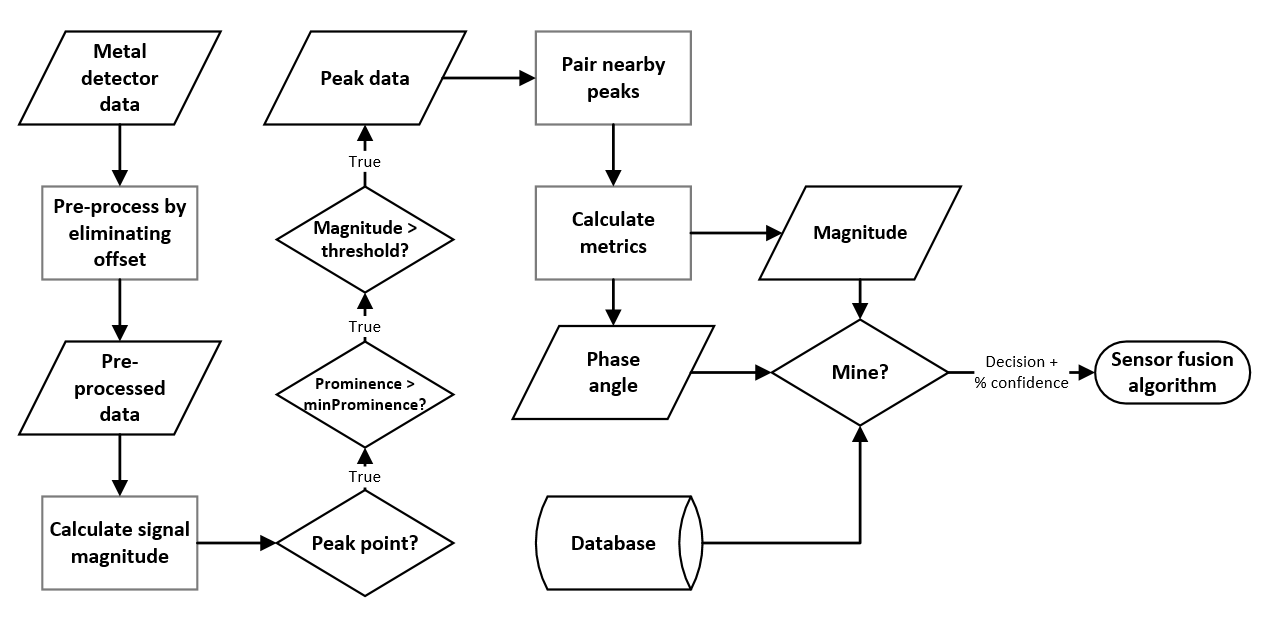
\includegraphics[width=\textwidth]{4-DetailedDesign/MDflow.PNG}
\centering
\caption{Algorithm to process the metal detector raw data}
\figlabel{MDflow}
\end{figure}

\Figref{MDalg} shows the phase loop plot that identifies the peaks of the signals, as well as the magnitude plot used to identify these prominent peaks.

\begin{figure}[ht]
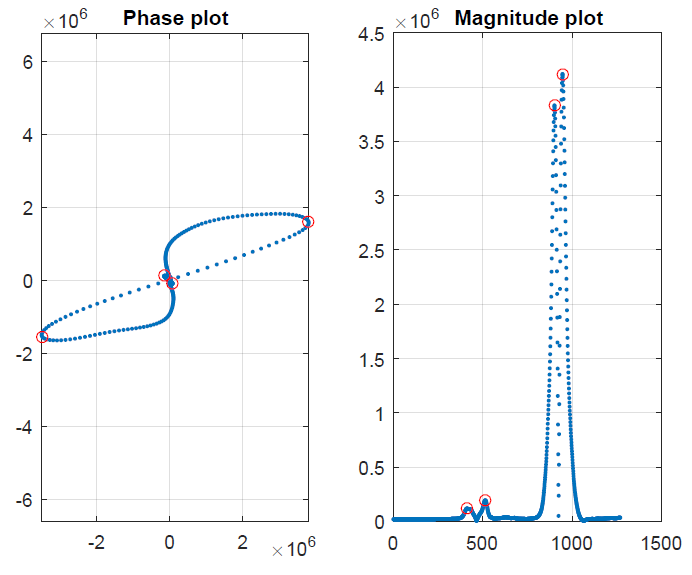
\includegraphics[width=0.6\textwidth]{4-DetailedDesign/phase.PNG}
\centering
\caption{Output of metal detector algorithm} 
\figlabel{MDalg}
\end{figure}

After initial tests of the metal detector data, another set of preliminary testing of the metal detector was completed at two different outdoor sites in order to gather data sets for the algorithm to process and to determine the parameters the metal detector will use in further testing. Further details of these tests are referred to \Chapref{testProcedureApp}. 

The data was processed by the algorithm above and the results found that the APM landmines were distinguishable from ten out of twelve clutter objects. The two that were similar to the APM were the steel beam and gutter section with average phase angles of -60 and -51 degrees and average magnitudes of 2.61E+05 and 3.92E+05, respectively. These values were within the phase angle range of the APM between -67 and -40 degrees, and magnitude between 6E+04 and 5E+05. The AT mines were able to be differentiated from all clutter objects. 

It was decided from these tests that only the centre panel (channel 2) and the lowest frequency of 1.5 kHz are to be used in further tests as suggested by Minelab and supported by literature \parencite{bruschini02}. The results contributes to the development of a database to be able to determine the percentage confidence of an object being a mine. The output metric values, such as phase angle and magnitude are stored in this database, which is used as part of the sensor fusion algorithm. 

\textcolor{red}{\textbf{General comment for all figures: shows/label items in figure (post-process), make sure font size is at least as large as the text, assume it will be in black and white (i.e. don't refer to colours in the figure, number or label things instead)}}

\subsection{GPR algorithm}
The processing of the GPR data is completed using an algorithm similar to the metal detector algorithm, except the metrics of interest are the feature width, feature depth and A-scan characteristics. These steps are shown on the flowchart in \Figref{GPRflow}. One key difference is that there are two pre-processing stages, which is due to the lower signal to noise ratio required in identifying subsurface objects.  In the first, an average is taken over all the A-scans, and this offset is removed from the data set. This results in a smoothing of horizontal lines seen in the raw scan when compared to the processed image. The next step is to find the A-scan with the lowest magnitude and remove this reference signal from all the data. This results in smoothing of the signal in the vertical direction.

\begin{figure}[ht]
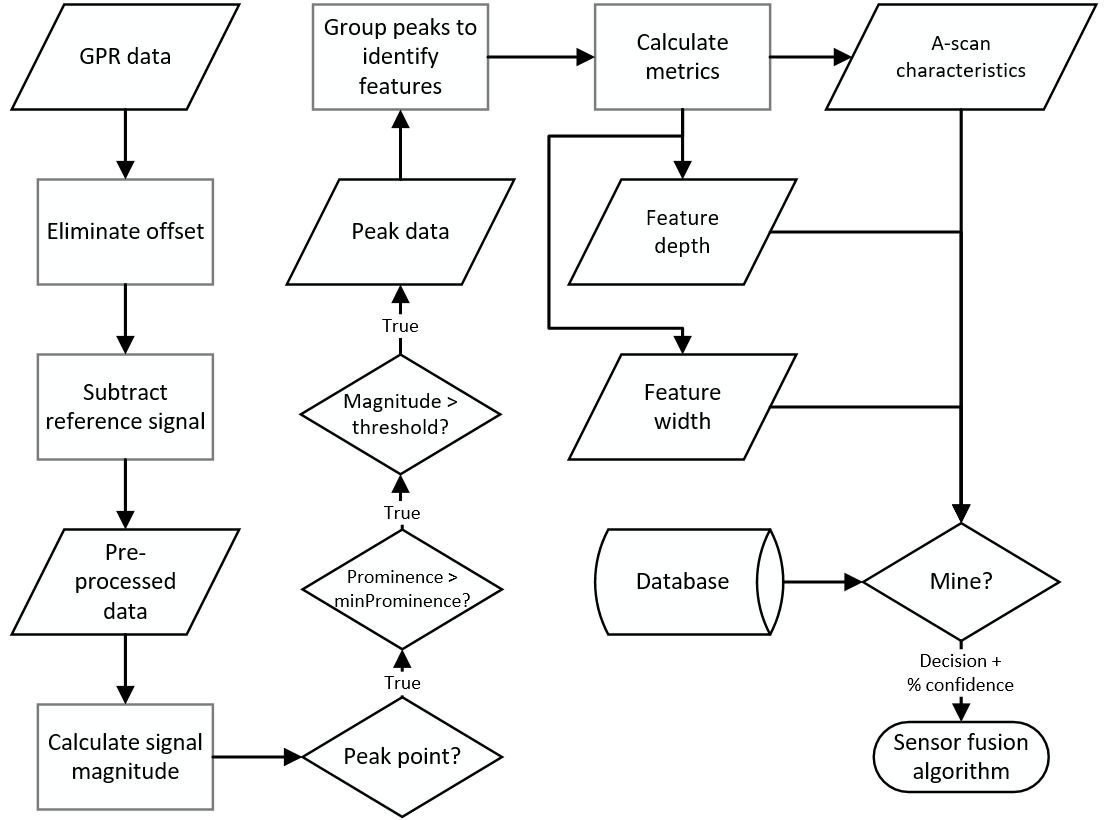
\includegraphics[width=\textwidth]{4-DetailedDesign/GPRflow.PNG}
\centering
\caption{Algorithm to process the GPR raw data}
\figlabel{GPRflow}
\end{figure}

The signal peaks are then detected by comparing all the values within the object’s signature and identifying the minimum and maximum prominent peaks. These prominent peaks are grouped into their positions on the graph such that the width and depth can be identified. The width is calculated based on the values within the section of prominent peak range, and the depth is calculated from maximum prominent peak from signals at the top of the soil. \Figref{GPRalg} shows the features for three replica landmine signatures processed by the algorithm. The vertical black line references the centre for each landmine feature. The red circles show the feature width, and the feature depth is calculated from top of the soil to the horizontal black line, where the maximum magnitude signal of the feature occurs.

\begin{figure}[ht]
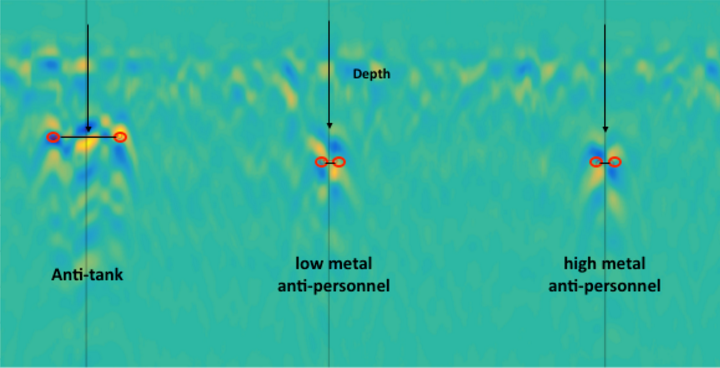
\includegraphics[width=0.7\textwidth]{4-DetailedDesign/GPRalg.PNG}
\centering
\caption{GPR B-scan of three mine after processed by algorithm}
\figlabel{GPRalg}
\end{figure}

The set of preliminary testing completed at the two outdoor test sites included GPR test scans in order to gather and compare this data with the metal detector data under similar conditions. These tests were also completed to confirm the frequency to be used for further GPR tests. The output metric values, such as feature width and depth are stored in the database similar to the metal detector used as part of the sensor fusion algorithm. 

After these preliminary test results were processed, the Bscan images from the 800 MHz and the 2 GHz frequency had a low signal to noise ratio as it detected more clutter or background signals in comparison. The lower 800 MHz frequency detected more clutter at a deeper depth, and the 2 GHz frequency detected clutter surrounding the target objects. Therefore, it was decided that the 1.4 GHz frequency is used for further tests as this provided the balance between penetration depth and frequency signal resolution received by the GPR.

The result from the data processed by the GPR algorithm found that there were three clutter objects that were similar to the APM and APC mines. These objects were the aluminium can, saucepan and gutter section with an average feature width of 11, 13 and 13, respectively. These values were within the feature width range of the APM and APC mines between 11 and 14. However, it was found that the feature depth of the landmines and clutter objects were distinguishable from each other. All of the AT mines were able to be differentiated from other objects. It is important to note that the other seven clutter objects were unable to be processed as there were insufficient data available from the preliminary tests due to inconsistencies in scanning. Regardless, the results from these output metrics, feature width and depth, will be used with the sensor fusion algorithm. 

\section{Sensor fusion}
The sensor fusion algorithm combines the results of the metal detector and GPR algorithms to produce a decision regarding the target, along with a confidence interval. This information is provided to the operator, who then decides how to proceed. Since the metal detector can only be used to detect metallic objects, it is anticipated that non-metallic objects are less likely to be detected, and will have a lower confidence interval. 

The algorithm starts with the phase angle output metric and if there is a phase angle value produced from the metal detector, it then compares this to the landmine data from the existing database. The object is then confirmed with the magnitude value to provide a confidence interval. If the phase angle or magnitude is zero or indistinguishable from the current database, it can be determined that the object is not metallic, thus, the GPR will then be used to scan over the object to confirm the feature width and depth. This data is then compared with the current database values. After producing a confidence interval of the object, the data is then sent through to the operator device.  

%%%%%%%%%%%%%%%%%%%%%%%%%%%
\todo[inline]{Moved from Results}
%%%%%%%%%%%%%%%%%%%%%%%%%%%

\textcolor{blue}{The phase angle and magnitude output from the metal detector may be used independently to confirm metallic landmines and clutter objects. The phase angle data may be analysed first as this is independent of the target depth. If the algorithm detects it as a landmine, the magnitude is then used to confirm the object as shown in \Tabref{mdMetrics}. Similarly, the feature width for the GPR data may be analysed first, followed by a confirmation of the object using the feature depth. The data from these results are stored in a database to be used by the sensor fusion algorithm. The output metric values from the phase angle, magnitude, feature width and depth are then retrieved by the algorithm to be able to compare the current scans with the relevant values. This then produces a percentage confidence of the scanned object of being a landmine. As discussed in scenario of operations, the platform stops when it has detected an object and data is sent wirelessly from the platform’s central computer system to the tablet device. The operator is then able to effectively decide to remove the object based on the processed data it receives from the central computer.} 

\textcolor{red}{More details about what info the operator receives, and what they should do with this info (link back to scenario of operation: detection is made, quad bike stops, operator decides if it's worth checking out, send in the demining team, clear the mine, proceed (?)) - See paragraph above in blue}

\section{Platform modifications}
\seclabel{detailedmodifications}
A visual inspection and individual tests of each of the subsystems revealed a number of hardware and software issues. Due to this changes were made to the electronics and control, steering, braking, gearing and positioning systems. No changes were made to the throttle and wheel encoder systems as they appeared to be operating correctly. \textcolor{red}{Need schematics/diagrams to support this section}
\subsection{Electronics and control}
\seclabel{modificationElec}
In accordance with the scheme detailed in the Concept Design, the low level I/O for controlling the remote platforms sensors and actuators was to be deferred to a microcontroller. The existing electronics within the quad bike had a central microcontroller fulfilling this same purpose. The existing microcontroller, a Motorola DragonBoard was however deemed inappropriate for the continued development of the platform due to obsolescence. The selected replacement microcontroller was to be Arduino based, to make the most of the more modern microcontroller system and the wide community support provided for the open source platform. An Arduino Mega2560 was chosen over other models due to the increased number of serial communication ports available and the increased potential for I/O expansion. 

The remainder of the existing electronics were purpose built for the quad bike either by the University of Adelaide electronics workshop or by previous students involved with the quad bike project. Following discussions with the workshop staff and a review of the schematics the workshop constructed items were deemed appropriate for reuse. The items constructed by previous students were largely made redundant by the introduction of the more modern Arduino controller and so they were discarded. Electronics items retained from the previous design were the regulated switched mode power supply, the relays and relay control board, the wheel encoder signal converter, the limit switch breakout board and the opto-isolator. 


\subsection{Steering}
\seclabel{modificationSteering}
Initial testing of the steering system demonstrated that the existing arrangement was not adequate for providing the required torque to steer the quad bike. Under stationary tests with the quad bike on a raised stand, the steering motor performed as expected, however under loading the motor would quickly draw a greater current than the regulated 24 V power supply could deliver. This resulted in the motor enabling a brake mode, ceasing all motion and losing track of the current encoder position making positional accuracy and repeatability impossible. To remedy this, a new 24 V regulated power supply was sourced which was capable of delivering the maximum current the steering motor could draw – 19 A, a significantly larger unit than the previous 2.5 A supply. The result of this replacement was the completion of all further testing without experiencing current supply issues. The steering motor is now capable of turning the wheels over the full range of motion while under the load from the entire weight of the quad bike, without losing positional accuracy.
%%photo? of the power supplies?
\subsection{Brakes}
\seclabel{modificationBrakes}
The original brake system (shown in \Figref{brakemodifications} a) incorporated a limit switch and strain gauge to determine if the brake actuator was extended. The limit switch limited the brake motion at the extreme limit and the strain gauge dictated the brake intensity and ensured the brake lever was not being over strained. A high level testing set-up was carried out by requesting certain braking intensities and measuring two values: travel distance of the actuator arm and the retarding torque on the wheel provided by the brake. It was found that the brake intensity fluctuated by 15 percent which would result in inconsistent stopping distances and speeds. The tests lead to the redesign of the brake measurement for greater accuracy. Improved braking accuracy was achieved through the use of a linear transducer type PZ34-A-125 being installed alongside the actuator (shown in \Figref{brakemodifications} b). This transducer allowed for the position of the brake actuator to be known with sub-millimetre accuracy. Knowing the position of the actuator arm allows for accurate and uniform brake intensities and thus, braking distances.
\begin{figure}[ht]
\centerline{
\begin{tabular}{cc}
\subfloat[Before]{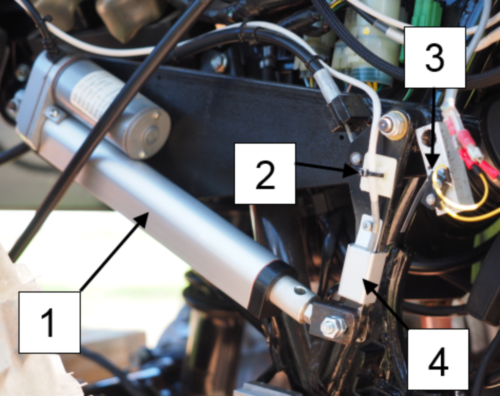
\includegraphics[width=0.45\textwidth]{4-DetailedDesign/BrakesOldLabelled.png}} 
& \subfloat[After]{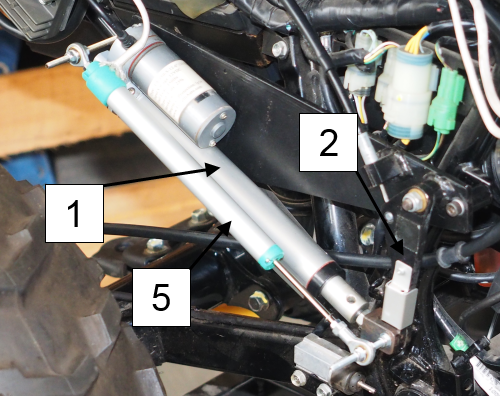
\includegraphics[width=0.45\textwidth]{4-DetailedDesign/BrakesNewLabelled.png}}\\
\end{tabular}}
\caption[Braking system before and after modification]{Braking system before and after modification, showing the linear actuator (1), brake level (2), limit switch (3), strain gauge (4), and linear transducer (5)}
\figlabel{brakemodifications}
\end{figure}

\subsection{Gears}
\seclabel{modificationGears}
As highlighted in the platform requirements, forwards and reverse motion is required for the desired mission profile. A linear actuator in conjunction with two linear potentiometers were used to move the gear selector lever. The linear potentiometers measured the forwards or backwards motion of the actuator and dictated the limits of the motion. Neutral was the position in the middle of the sensors while Drive and Reverse were to the left and right respectively. Selecting Drive or Reverse resulted in the actuator pushing the gear lever to a point until the hall effect sensor reached a certain value and the arduino ordered the actuator to stop. For correct operation of the system the potentiometers were replaced. It was also found that the tab which interacts with the hall effect sensors would slip out of place due to the springs which held it to the actuator. A larger tab was installed to make this an impossibility.
\begin{figure}[ht]
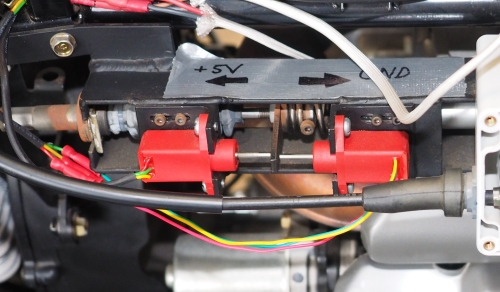
\includegraphics[width=0.6\textwidth]{4-DetailedDesign/gearSetup.JPG}
\centering
\caption{Gear setup showing hall effect sensors in red in front of the gear actuator} \figlabel{gearSetup}
\end{figure}
\subsection{Positioning}
\seclabel{modificationPositioning}
No positioning system was initially present in the quad bike. For implementation of the designed Kalman Filter (see \secref{positioningSystem}) a uBlox NEO-6M GPS and GY-87 10-DOF IMU were installed into the system. The selected units are shown in \Figref{gpsIMU}. The uBlox NEO-6M has an update rate of 1 Hz and a horizontal position accuracy of 2.5 meters \parencite{ublox2011}. The GY-87 chip includes an MPU-6050, HMC5883L, and a BMP180. The MPU-6050 combines a 3-axis gyroscope with sensitivity of +/- 2g, and 3-axis accelerometer with a sensitivity of 250 \degree/s \parencite{invensense2013}. The HMC5883L compass and BMP180 pressure sensor were not used as part of the positioning system.

\begin{figure}[ht]
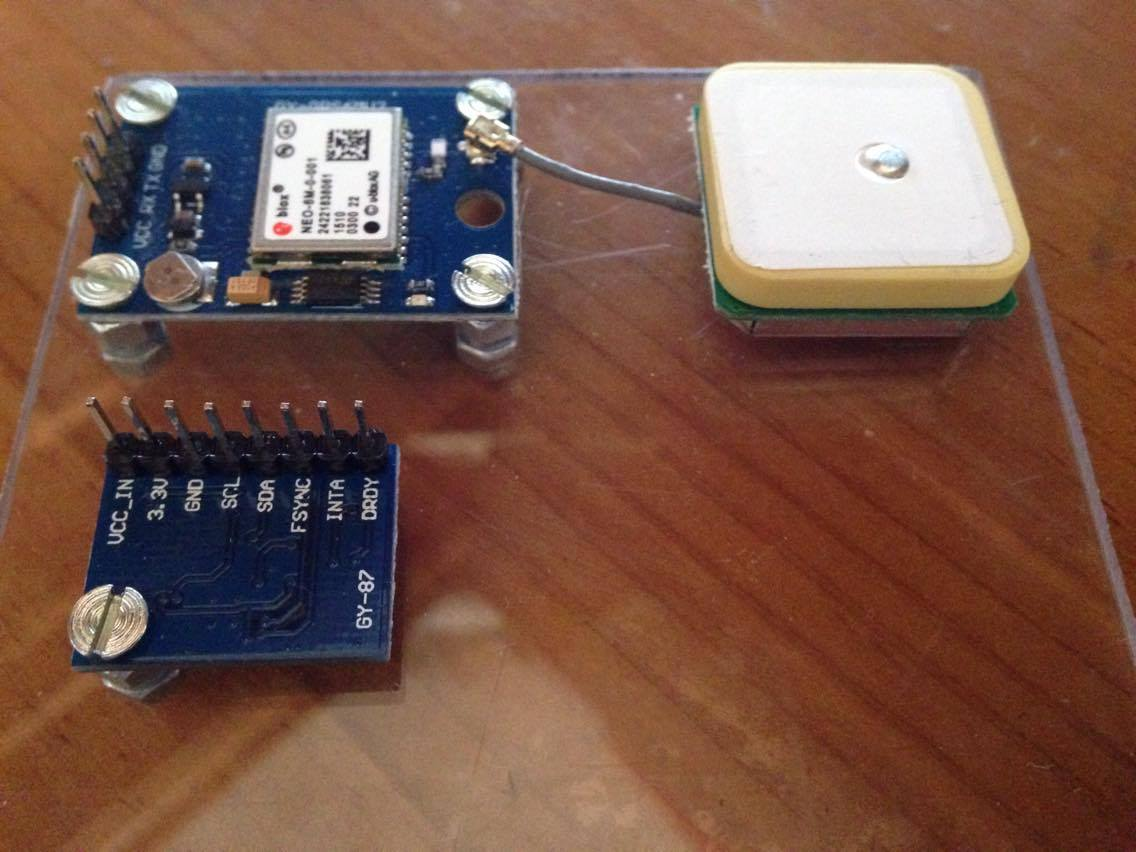
\includegraphics[width=0.6\textwidth]{4-DetailedDesign/Positioning.jpg}
\centering
\caption{(Top) UBlox GPS and receiver and (bottom) GY-87 10DOF IMU} \figlabel{gpsIMU}
\end{figure}

\section{Navigation}
\seclabel{detailednav}
Platform navigation is primarily handled via waypoints. After a region is selected by a user it is broken down into a series of waypoints which the quad bike will attempt to follow. In the alternate use case, the user will specify a path directly and the navigation system will operate directly on these waypoints.

\subsection{Region subdivision}
\seclabel{detailedregionsubdivision}
The waypoints are generated from a zone of interest to facilitate the autonomous surveying of areas that are suspected to contain landmines. This zone must be capable of being user defined to match real world boundaries. The algorithm used to generate these waypoints is a modified linescan algorithm which will be tuned to output scanlines of the same width as the equipment's scan width, defined as 3 meters in the specifications.

To allow for complex polygonal zones to be entered by the user, the original user-defined polygon boundary is split into a series of convex hulls, simplifying the line scanning algorithm. The split of the user polygon is shown in \Figref{wayPointGeneration}, where the user-defined polygon is outlined in bold blue and the series of generated convex search regions are shaded within. The black path shows the output of the linescan algorithm starting at the origin (marked by the red dot in the south-east corner), and ends at the second red dot at the far end of the path. 
\begin{figure}[ht]
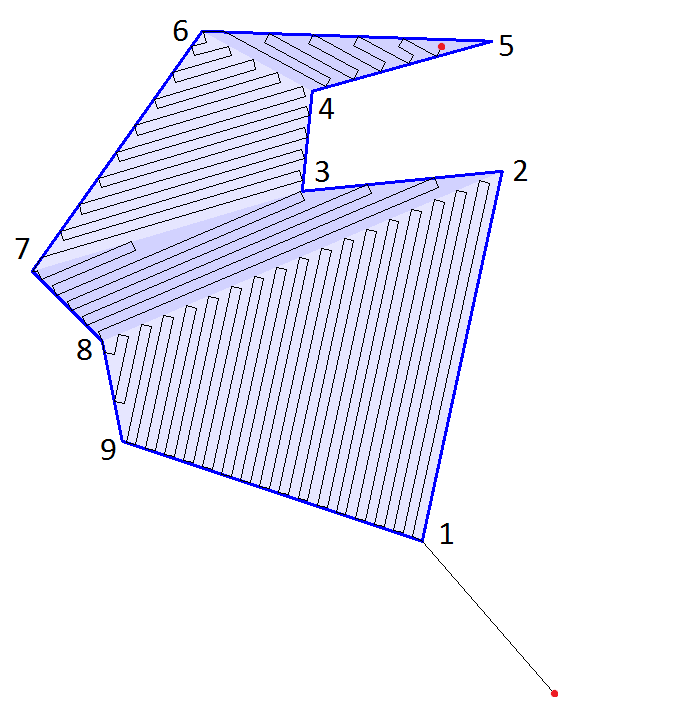
\includegraphics[width=0.5\textwidth]{4-DetailedDesign/lineScanAlgorithm2.png}
\centering
\caption{Output of preliminary waypoint generation algorithm} \figlabel{wayPointGeneration}
\end{figure}
The linescan algorithm searches for the nearest corner from the nearest convex polygon and begins plotting successive alternating scanlines through the polygon. After a convex polygon has been completely covered, the linescan algorithm connects to the next nearest corner of the next nearest polygon and the process continues. This system allows for multiple user defined regions to be connected and autonomously scanned in a single pass. Due to the way the region subdivision takes place the only radius of curvatures present are either zero (corner), or infinite (straight line) shown in \Figref{curvatures}.
\begin{figure}[ht]
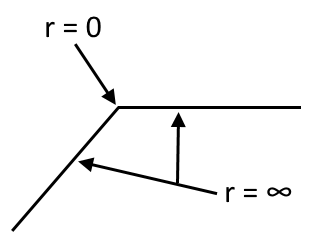
\includegraphics[width=0.6\textwidth]{4-DetailedDesign/radiusOfCurvatures.png}
\centering
\caption{Radii of curvatures present in region subdivision \textcolor{red}{Maz didn't like this}} \figlabel{curvatures}
\end{figure}
For low curvature path following Pure Pursuit is used (\secref{lowcurvefollowing}). Low curvature is defined as any path with a radius of curvature greater than that of the minimum turn radius of the quad bike, ie. a radius of curvature greater than 3.14 meters. The quad bike's maximum steering angle of 24 degrees restricts it from making any turn sharper than this. For a radius of curvature of zero, the pure pursuit method breaks down due to turn angle limitations on the quad bike and another turning method is required.

\subsection{Low curvature path following}
\seclabel{lowcurvefollowing}
The low curvature path tracker works through determining a steer angle that connects an arc from the centre point of the non steering wheel axle to a goal point on the path (refer to \Figref{purePursuitGeom}).  The goal point ($g_x, g_y$) acts as an intermediate waypoint and is determined from a look-ahead distance $l_d$. The angle, $\alpha$, can be related to the geometry using the law of sines,
\begin{align}
\frac{l_d}{\sin(2\alpha)} &= \frac{R}{\sin(^{\pi}/_2-\alpha)},\\
\frac{l_d}{2\sin(\alpha)\cos(\alpha)} &= \frac{R}{\cos(\alpha)},\\
\frac{l_d}{2\sin(\alpha)} &= R.
\shortintertext{Then the steer angle, $\delta$, can be determined from the geometry shown in \Figref{geometricBicycleModel} where}
R &= \frac{l_d}{2\sin(\alpha)},
\shortintertext{and the pure pursuit controller is given as}
\delta &= \tan^{-1}\Bigg(\frac{2L\sin(\alpha)}{l_d}\Bigg)
\end{align}
where $\alpha$ and thus $\delta$ will be functions of time and thus will be calculated in real time. The goal point is determined as a result of further path subdivision discussed in \secref{pathsubdivision}.
\begin{figure}[ht]
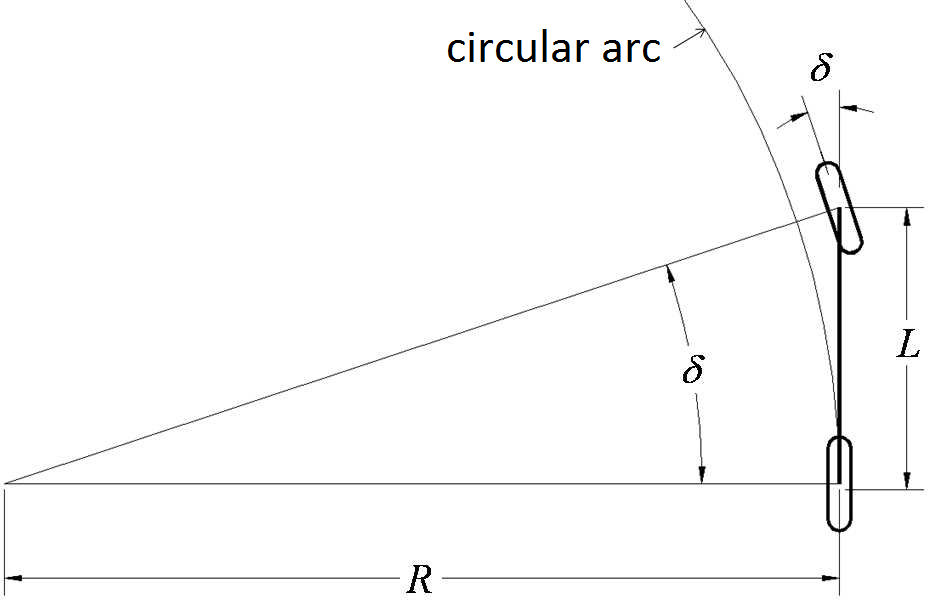
\includegraphics[width=0.7\textwidth]{4-DetailedDesign/Geometric_Bicycle_Model.png}
\centering
\caption[Geometric bicycle model]{Geometric bicycle model \parencite{snider2009}} \figlabel{geometricBicycleModel}
\end{figure} 

\subsection{Turning the platform a specified angle}
\seclabel{turningspecifiedangle}
For the quad bike to not stray more than 0.5 meters from the path, as defined in the project requirements, turning procedures were incorporated at path points of zero radius of curvature. In these situations one of two methods were used to turn the angle, a simple turn, or an extended 3-point turn (N-point turn) to some number of required points, both shown in \Figref{turnTypes}. 

\begin{figure}[ht]
\centerline{
\begin{tabular}{ccc}
\subfloat[User defined path]{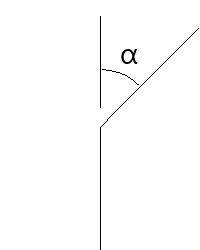
\includegraphics[width=0.25\textwidth]{4-DetailedDesign/noturn.png}} 
& \subfloat[Simple turn]{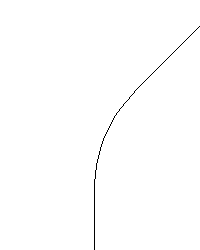
\includegraphics[width=0.25\textwidth]{4-DetailedDesign/simpleturn.png}}
& \subfloat[N-point turn]{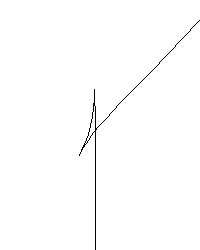
\includegraphics[width=0.25\textwidth]{4-DetailedDesign/npointturn.png}}\\
\end{tabular}}
\caption{Turning types}
\figlabel{turnTypes}
\end{figure}

The turn type used at any point is determined by a user set threshold of angles. The angle values may be determined based on how quickly the quad bike should scan the area, as an N-point turn requires several changes of direction and thus more time, or how accurate to the path the quad bike should remain, as the simple turn will result in the quad bike deviating from the user path. To test both scenarios in the Virtual Platform and during live testing, the thresholds were defined as follows:
\begin{itemize}
\item $\alpha <$ 40\degree: Simple turn
\item $\alpha \geqslant$ 40\degree: N-point turn
\end{itemize}

The geometry of the simple turn is shown in \Figref{simpleTurnGeometry} where the solid bold line and dashed bold line represent the user defined path and the modified region of the path, respectively. We can visually see that to reduce the deviation from the user defined path, d should be kept to a minimum.
\begin{figure}[ht]
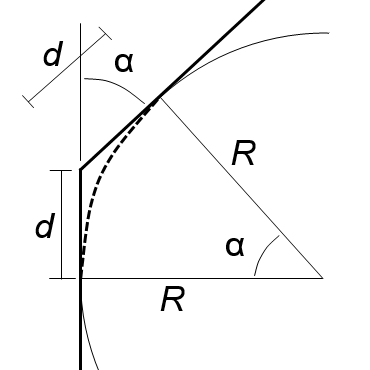
\includegraphics[width=0.4\textwidth]{4-DetailedDesign/simpleTurnGeometry.png}
\centering
\caption{Simple turn geometry} \figlabel{simpleTurnGeometry}
\end{figure} 
From \Figref{simpleTurnGeometry} we get:
\begin{align*}
d = R \tan{\frac{\alpha}{2}}\\
\end{align*}
To minimise $d$, the turn radius, $R$, should be minimised. To minimise the turn radius the turn should be executed at maximum turn angle, or with $\delta$ equal to 24\degree. Mapping waypoints along the simple turn is covered further in \secref{pathsubdivision}.

Geometry for the N-point turn is very similar to that of the simple turn and is shown in \Figref{nPointTurnGeometry}. Again, the solid bold line and dashed bold line represent the user defined path and the modified region of the path, respectively. The grey box is the quad bike position and the grey dashed lines are the scanned swathe from the sensor suite.
\begin{figure}[ht]
\centerline{
\begin{tabular}{cc}
\subfloat[Arc geometry]{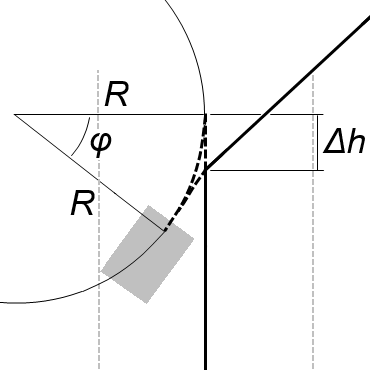
\includegraphics[width=0.4\textwidth]{4-DetailedDesign/nPointTurnGeometry.png}} 
& \subfloat[Turn points]{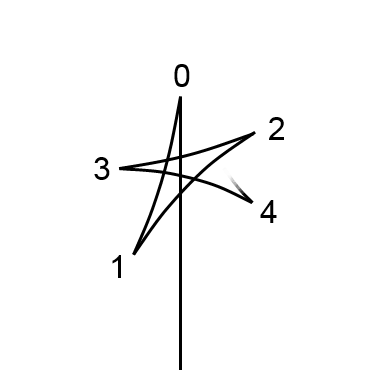
\includegraphics[width=0.4\textwidth]{4-DetailedDesign/nPointTurnNumbered.png}}\\
\end{tabular}}
\caption{N-point turn geometry}
\figlabel{nPointTurnGeometry}
\end{figure}

Throughout the N-point turn the quad bike must remain within the grey dashed lines else it would be traversing un-scanned terrain, risking the detonation of landmines. By analysing a 180 degree N-point turn in a 3 meter swathe, a template is constructed, and for any turn angles of less than 180 degrees the turn algorithm exits early, once the desired turn angle has been reached. The specific algorithms to achieve this are discussed further in \secref{pathsubdivision}. The template, shown in \Tabref{npointTurnTemplate}, matches each point in the turn with an angle corresponding to the angle at which the quad bike touches the edge of the swathe. In \Figref{nPointTurnGeometry}a, the quad bike is touching the edge of the swathe at position 1, 26.7\degree. Accumulative error here is not an issue as this is the ideal path that the quad bike would follow, and any quad bike deviation error is corrected for by aiming for the ideal path point.
\begin{table} [ht]
\centering
\caption{N-point turn template}
\tablabel{npointTurnTemplate}
\begin{tabular} {r c c c c c c c c}
\toprule
Turn point & 0 & 1 & 2 & 3 & 4 & 5 & 6 & 7 \\ \midrule
Heading (\degree) & 0 & 26.7 & 60.5 & 77.3 & 95.6 & 113.9 & 130.8 & 180 \\
$\Delta h$ required (m) & 0 & 1.46 & 0.09 & 0.44 & 0.37 & 0.11 & 0.62 & -1.18 \\ \bottomrule
\end{tabular}
\end{table}
At the completion of the turn, the quad bike is not guaranteed to line up with the next segment of the path. A distance, $\Delta h$ is added to the end of the previous line segment to correct for this. $\Delta h$ is also determined from ideal geometry, and in real time by interpolating from the template shown in \Tabref{npointTurnTemplate}.

\subsection{Path subdivision}
\seclabel{pathsubdivision}
The goal of the path subdivision step is to provide intermediate, or 'goal', waypoints for the quad bike to navigate towards. The subdivision is completed by cycling through the user defined path, constantly repeating a two step process: 
\begin{enumerate}
\item Subdivide the straight line segment
\item If there is a next line segment, conduct a turn and align with it
\end{enumerate}
Straight line segments are subdivided through linear interpolation and adding intermediate waypoints at some user defined distance. In the Virtual Platform, and for testing, a distance of 0.2 meters is used.

For each of the turns, the algorithm to deduce the locations of the modified path is a fast, vector based process. For more detail on the algorithms used to achieve this see \chapref{pathSubdivisionDetail}. The final result of the subdivision process is shown in \Figref{pathSubdivisionBeforeAfter}.
\begin{figure}[ht]
\centerline{
\begin{tabular}{cc}
\subfloat[Input: user or region defined path]{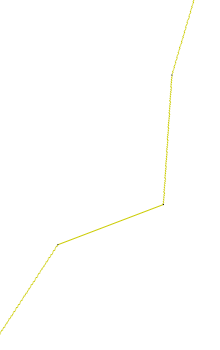
\includegraphics[width=0.3\textwidth]{4-DetailedDesign/rawpath.png}} 
& \subfloat[Output: subdivided path with calculated turns]{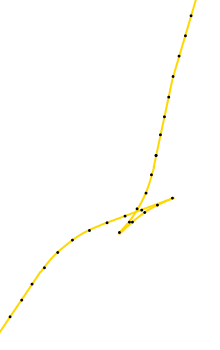
\includegraphics[width=0.3\textwidth]{4-DetailedDesign/subdividedpath.png}}\\
\end{tabular}}
\caption{Path subdivision input and output \textcolor{red}{The lines are quite faint, can we make them darker/thicker}}
\figlabel{pathSubdivisionBeforeAfter}
\end{figure}

\subsection{Positioning system}
\seclabel{positioningSystem}
The requirements for the positioning system were set primarily by the virtual platform (see \secref{detailedVP}). Two requirements were defined for the design, low positional drift and high accuracy. The drift is the speed at which the cartesian position moves relative to the real quad bike position and accuracy is the distance error of the positioning system from the real quad position. The maximum allowable drift for the system was defined as 0.2 m/s, speeds exceeding this resulted in irregular steering motor fluctuations either side of the desired steering angle. The minimum allowable accuracy for the position was defined as 0.5 m as set in the project specifications.

To satisfy these characteristics an Extended Kalman Filter (EKF) was employed to fuse the data from two positional sources, a GPS and IMU, and quad bike kinematic equations. It is capable of taking in to account the noise and inaccuracies from multiple measurements to produce an output which is likely to be more accurate than each of the individual readings. The EKF is defined as follows:
\begin{align*}
\shortintertext{Prediction Equations:}
&\bar{\mu_t} = g(u_t, \mu_{t-1}) + \delta_t\\
&\bar{\Sigma_t} = G_t\Sigma_tG_t^T + R_t\\
\shortintertext{Update Equations:}
&z_t = h(\mu_t) + v_t\\
&K_t = \bar{\Sigma_t}H_t^T(H_t\bar{\Sigma_t}H_t^T + Q_t)^{-1}\\
&\mu_t = \bar{\mu_t} + K_t(z_t-h(\bar{\mu_t}))\\
&\Sigma_t = (I - K_tH_t)\bar{\Sigma_t}
\end{align*}
\textcolor{red}{\textbf{Label equations}} Where the state vector, $\mu_t$, holds the positional information ($x, y, \theta$) in a 3x1 matrix. The EKF is calculated in two steps, a prediction step and an update step. The prediction step uses kinematic equations to update the position of the quad bike based on physical observations. In the case of the quad bike, readings of the velocity, steering angle and time-step are taken, then geometry is used to calculate where its updated position would be. The update step then uses information obtained through sensors to correct for any error that may be present in the prediction step. This is achieved by modelling positions as a Gaussian distribution and weighting them according to their reliability. Gaussian distributions are shown as covariance matrices, $R_t$ for the prediction step and $Q_t$ for the update step, and the weighting is the Kalman Gain, $K_t$. The predicted covariance matrix, $\Sigma_t$, can then be determined. As we know the starting position and heading of the quad bike through user input, $\Sigma_t$ is initialised as a 3x3 zero matrix.

The geometry of the kinematic equations used are shown in \Figref{quadKinematics}. From the geometry we get:
\begin{align*}
&R = \frac{L}{tan\ \delta}\\
&\phi = \frac{V\Delta t}{R}\\
&y_q = Rsin\phi\\
&x_q = R(1-cos\phi)
\shortintertext{where $R$ is the turn radius, $L$ the wheelbase, $\delta$ the steer angle, $V$ the velocity, $\Delta t$ the time step, and ($x_q, y_q$) is the local change in position. Then in the global frame we have:}
&x_G = y_qsin\theta + x_qcos\theta\\
&y_G = y_qcos\theta + x_qsin\theta\\
&\theta = \theta + \phi
\end{align*}
\begin{figure}[ht]
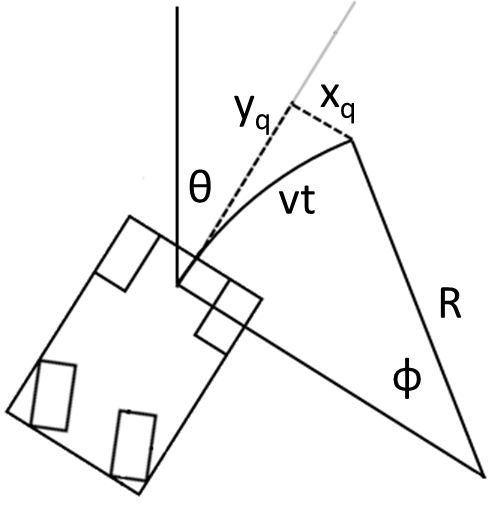
\includegraphics[width=0.5\textwidth]{4-DetailedDesign/quadbikeKinematics.png}
\centering
\caption{quad bike Kinematics} \figlabel{quadKinematics}
\end{figure} 
so the prediction equation for $\bar{\mu_t},\ g(u_t,\ \mu_{t-1})$ becomes:
\[
g(u_t, \mu_{t-1}) =
\begin{bmatrix}
	x_G + y_qsin\theta + x_qcos\theta\\
    y_G + y_qcos\theta + x_qsin\theta\\
    \theta + \phi
\end{bmatrix}
\textrm{, } G = \frac{\partial g_i}{\partial x_j} =
\begin{bmatrix}
    1	&	0	&	y_qcos\theta - x_qsin\theta\\
    0	&	1	&	-y_qsin\theta - x_qcos\theta\\
    0	&	0	&	1
\end{bmatrix}
\]
This needs to be recalculated at each prediction step as well as it's Jacobin, $G$. The process noise for the prediction, $\delta_t$, is represented by a Gaussian distribution with covariance $R$.
\[
R =
\begin{bmatrix}
    \sigma_x^2	&	0	&	0\\
    0	&	\sigma_y^2	&	0\\
    0	&	0	&	\sigma_\theta^2
\end{bmatrix}
=
\begin{bmatrix}
    (0.025 \times V\Delta t)^2	&	0	&	0\\
    0	&	(0.025 \times V\Delta t)^2	&	0\\
    0	&	0	&	(0.97 \times V\Delta t)^2
\end{bmatrix}
\]
Where $\sigma_x, \sigma_y, \textrm{and } \sigma_\theta$ are based on the accuracy of readings given by the velocity and steer angle sensors on the quad bike. Testing (see \secref{testingwheelencoder}) showed the error in distance, ($\sigma_x, \sigma_y$), to consistently vary within 0.5 m for every 20 m travelled, or 0.025 m/m. Since the heading is calculated based on the distance travelled and the turn angle, the error is also dependent on these factors. The steering motor is accurate to 1 degree of the true value due to initialisation and the error is maximum when at full lock due to the trigonometric function present in the turn angle equation below. The difference in turn angle at full lock when a 1 degree error is present is then:
\begin{align*}
&\Delta\phi = \frac{V\Delta t}{\frac{L}{tan\ 24}} - \frac{V\Delta t}{\frac{L}{tan\ 23}} = \frac{V\Delta t}{2.87} - \frac{V\Delta t}{3.02} = 0.017V\Delta t = 0.97\ \degree/m
\end{align*}
Positional and angular data from the GPS and angular data from the IMU are observed. In the case of the GPS, the EKF inputs are the observation matrix and its Jacobian:
\[
h(\mu_t) = \mu_t = 
\begin{bmatrix}
    x_{gps}\\
    y_{gps}\\
    \theta_{gps}
\end{bmatrix}
\textrm{, } H = \frac{\partial h_i}{\partial x_j} = 
\begin{bmatrix}
    1	&	0	&	0\\
    0	&	1	&	0\\
    0	&	0	&	1
\end{bmatrix}
\]
And an observation error modeled by a Gaussian distribution with covariance matrix $Q$:
\[
Q = 
\begin{bmatrix}
    \sigma_x^2	&	0	&	0\\
    0	&	\sigma_y^2	&	0\\
    0	&	0	&	\sigma_\theta^2
\end{bmatrix}
=
\begin{bmatrix}
    0.4^2	&	0	&	0\\
    0	&	0.4^2	&	0\\
    0	&	0	&	20^2
\end{bmatrix}
\]
\textcolor{red}{\textbf{label equations}} As the GPS drifts when stationary, positional data from this sensor is only used when the platform is at cruising speed, or when travelling in a forwards direction at 5 km/hr. Experimental data showed the GPS to be accurate within 0.4 m at this speed, and therefore the calculated heading accurate within ~20 degrees when measuring between subsequent points. This on its own is not accurate enough as it exceeds the desired positional accuracy.  

Therefore, the IMU is also used to correct the heading. As only one element of the state vector is being updated the matrix math is set up slightly differently. Experimental data shows the IMU has an error of approximately 2 degrees per 360 degrees travelled.
\[
h(\mu_t) = \mu_t = 
\begin{bmatrix}
    \theta + \Delta \theta_{imu}
\end{bmatrix}
\textrm{, } H = \frac{\partial h_i}{\partial x_j} = 
\begin{bmatrix}
    0	&	0	&	1
\end{bmatrix}
\]
And an observation error modeled by a Gaussian distribution with covariance matrix $Q$:
\[
Q = 
\begin{bmatrix}
    \sigma_\theta^2
\end{bmatrix}
=
\begin{bmatrix}
    (\frac{2}{360}\Delta \theta_{imu})^2
\end{bmatrix}
\]
With the inputs calculated a new estimate covariance, $\Sigma_t$, and position estimate, $\mu_t$, is outputted to be used in the next iteration of the algorithm. 

\section{Automation}
\seclabel{detailedautomate}

As part of the platform requirements, full autonomy of the vehicle was required. For the quad bike this meant being able to operate each of the subsystems, steering, throttle, gears, and brakes, remotely without human interaction as well as knowing state information about the quad bike including the speed, position and heading. To achieve this the quad bike uses a series of actuators and motors in conjunction with an Arduino control board to operate the subsystems in place of human interaction.

\subsection{Automation software}
\seclabel{detailedautosoftware}
Direct communication with the actuators is handled through an Arduino microcontroller. Any desired commands are sent from the desktop navigation software to the Arduino where final checks are in place to ensure incorrect operation does not take place. The code structure, shown in \Chapref{arduinoCodeChart}, uses individual control loops which are executed once each loop for each of the actuators. The control loops serve three purposes:
\begin{enumerate}
\item Ensure the desired position is within the actuator bounds
\item Ensure other actuators and/or sensors are in appropriate positions
\item Move the actuator to the desired position
\end{enumerate}
Some dependencies are present from one actuator to another. These include the gear actuator with the brake and throttle actuator, the brake actuator with the throttle actuator, and the throttle actuator with the brake actuator.

The gear actuator should only move if three conditions are satisfied. Firstly, the quad bike's velocity should be zero else unknown circumstances between gear changes may arise. Secondly, throttle percentage should be zero else uncontrolled accelerations may arise and lastly, the brakes should be applied to provide control of the quad bike during gear changes.

The brake actuator should not be applied unless the throttle percentage is zero. If the brakes are applied when throttle exists, the throttle is set to zero and the brakes are applied. Conversely, the throttle should not increase if the brakes have been engaged. Braking takes precedence over throttle and so the requested throttle change is ignored.

\subsection{Subdivided path following}
\seclabel{automationpathfollowing}
As discussed in \secref{pathconcept} and \secref{detailednav}, Pure Pursuit is used as the path following algorithm to turn towards the next goal point in the path. When the quad bike is within a specified look-ahead distance from the goal point, the point is incremented along the path and the process continues. This is true for all cases except when there is no next point and the path navigation is complete, or during N-point turn manoeuvres where complex navigation is required.

Due to the mixture of navigation complexities three navigation states were employed, NAV\_STOP, NAV\_CRUISE, and NAV\_TURNINBOUND. The quad bike performs different functions depending on the navigation state. If the current state is NAV\_STOP, the quad bike applies the brakes and stops. This would be used in the case of an emergency or landmine detection. NAV\_CRUISE is the basic Pure Pursuit algorithm; steer to the goal point and when within the given look-ahead distance, increment the path point.

The navigation software is able to detect an inbound turn via the distances between the current and next path points. If the distance to the next path point is less than the distance to the current path point, we know a point in the N-point turn is approaching and the navigation state is changed to NAV\_TURNINBOUND. When this is the case, the path point is not incremented until one of two possibilities occur; 1. the quad bike comes within a user specified radial tolerance of the point or 2. the quad bike is no longer converging on the point. For testing and in the virtual platform, a radial tolerance of 0.2 m was used. When one of the two possibilities returns true, the navigation state is reset to NAV\_CRUISE. The process starts again and if more points are present in the N-point turn, the navigation state will be set to NAV\_TURNINBOUND once again. The direction of travel is determined based on the location of the goal point relative to the quad bike. If the goal point lies in front of the quad bike, the forwards gear is selected, and if the goal point is behind the quad bike, the reverse gear is selected.

\section{Sensor mount}
%\subsubsection{Final sensor mount design}
For the final design for the sensor mount to adhere to all the sensory requirements, design tests were required to be conducted. These tests were necessary to test for variations in ground clearances and vibrational interference from the Quad bike during operation. Testing for these were carried out using the Finite Element Analysis (FEA) method and engine run tests on the quad bike with attached accelerometers. FEA was used to test vibrational harmonics and load carrying ability of the frame when subject to operational conditions while engine run tests were used to test the vibrational frequency of the operating quad bike. 
%The sensor mount, as described previously, is required to carry the sensory systems and mount them to the platform in a fashion that does not limit their functionality. The design process of the mount consisted of hand calculations followed, computer aided design and verification. 

\subsection{Structural analysis}
The sensor frame design was constructed in FEA. The FEA methods discretises a geometry into a finite number of elements connected together via nodes. Boundary conditions, loads and constraints as well as material properties are subject to the design and depending on the analysis type, a result can be interpreted that can be used to alter and fine tune the design.  To properly and accurately model the frame, 3D elements were chosen to represent the geometry and a basic load test was conducted. This load test was conducted to ensure that the deflection of the mount when subject to the weight of the sensor systems would not interfere with the sensor requirements, and to check if the design was strong enough to support the weight.

The initial FEA analysis was used to determine the thickness of the required mount material as well as the support locations. It was found that using structural pine MGP10 a thickness of 70 x 35 mm provided adequate support and minimised deflection to less than 4 mm. The supports were chosen to be made from mild steel with square hollow sections with dimension 25 x 25 x 1.6 mm. The equivalent (von-Mises) stresses for both the frame and mild steel supports did not exceed their yield stresses of 10 MPa and 370 MPa respectively. \Figref{topframe} and \Figref{bottomframe} show the equivalent stresses experienced by the segmented parts \textcolor{red}{FEA pictures need to be larger, also maybe change colour scale so that it's easier to see in black and white}. 

\begin{figure}[ht]
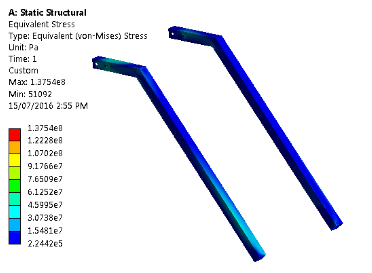
\includegraphics[width=0.7\textwidth]{4-DetailedDesign/top_frame.PNG}
\centering
\caption{Supports for sensor mount von-Mises stress} \figlabel{topframe}
\end{figure}

\begin{figure}[ht]
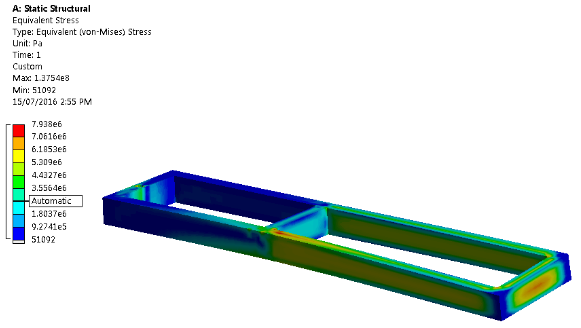
\includegraphics[width=0.7\textwidth]{4-DetailedDesign/bottomframe.PNG}
\centering
\caption{Structural pine frame von-Mises stress} \figlabel{bottomframe}
\end{figure}

Hand calculations were used to verify the results from FEA. An axial force of 334 MPa was calculated for the rear frame section and this corresponded to a force of 333.99 MPa from the FEA analysis showing that the results from FEA mimicked the real world results closely. 

The location of the sensors were dictated by each individual sensor requirements as discussed previously. The metal detector had to be in a 40 cm halo free of metallic objects while the GPR had to be as close to the ground as possible. \Figref{finalSensorFrameDesign} shows the final frame design and attachment of the sensors. The metal detector was placed 45 cm in-front of the metal supports and the GPR to reduce the interference. The GPR was mounted as close as allowable to the metal detector to minimise the separation between the sensors, so that the amount of miss-alignment experienced during turns would be low.  

\begin{figure}[ht]
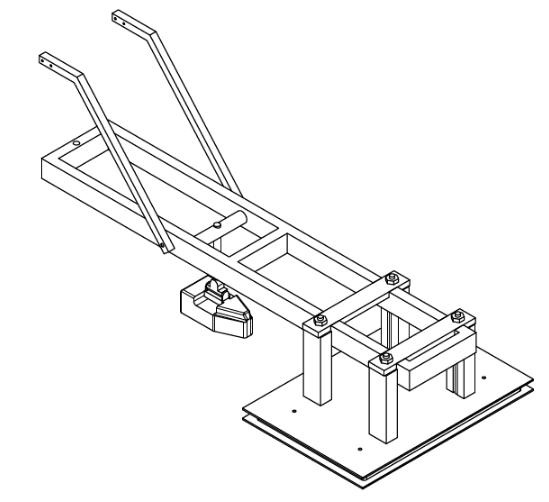
\includegraphics[width=0.6\textwidth]{4-DetailedDesign/frame.PNG}
\centering
\caption{Sensor mount frame design} \figlabel{finalSensorFrameDesign}
\end{figure} 

%A vibrational analysis was conducted to ensure that no frequency disturbances would be experienced by the sensors from the quad bike engine during operation. The analysis was also used to find the frame vibrations to ensure that the operational frequencies did not result in harmonics that could lead to unacceptable deflections.
\subsection{Vibrational analysis}
In order to determine the vibrational characteristics of the sensor mount while attached to the quad bike frame, a detailed analysis was undertaken. Initially, hand calculations for a simplified system were performed based on known theory. These results were then used to verify the results of simple FEA simulations. More complex FEA simulations were then performed, in order to more closely model the actual sensor mount. The next step will be to take experimental measurements, which should agree with FEA results within some margin of error. 
 \textcolor{red}{include some details about rough surface characterisation (from the back of the seminar slides) }
\subsubsection{Theoretical results}
While it is difficult to model the vibrational modes of a beam exactly, approximate analytical solutions for lower order modes may be obtained using classical methods. Two such methods are the Rayleigh and Dunkerly methods. The Rayleigh method considers the energy balance at the location of each beam mass element. A solution for the modes can be obtained based on knowledge of the static deflection. In general, the Rayleigh method provides an upper limit for the fundamental frequency. The Dunkerly method considers a force balance along the beam, which leads to the result that the overall modes are a superposition of the modes of the individual elements. The Dunkerly method generally provides a lower limit for the fundamental frequency.
\textcolor{red}{some references?}
Both methods were used to find the vibrational modes for three different configurations. The first configuration is a simple cantilever with self weight, the second is a massless cantilever with an end-loading, while the third is a cantilever with self-weight and an end loading.  \Tabref{theoreticalvibestable} shows the results for each of the different configurations and methods.

%\[
%Cross section: 35 x 70 mm    	Length: 1.5 m
%Density: 515 \frac{kg}{$m^3}   	Modulus of elasticity: 10.06 GPa 
%End load mass: 5 kg 			Beam mass = 1.8926 kg (calculated)

%\]

\begin{table} [ht]
\centering
\caption[Theoretical vibration results using Rayleigh and Dunkerly methods]{Theoretical vibration results using Rayleigh and Dunkerly methods for a 35 x 70 x 1500 mm beam in different configurations }
\tablabel{theoreticalvibestable}
\begin{tabular} {r c c}
\toprule
Configuration & f Dunkerly (Hz) & f Rayleigh (Hz)  \\ \midrule
Cantilever (1.9kg self weight) & 22.2097 & 34.0655  \\
Cantilever (massless, 5kg end load) & 6.7321 & 6.7321 \\
Cantilever (1.9kg self weight , 5kg end load) & 6.4427 & 6.8844 \\ \bottomrule
\end{tabular}
\end{table}

A cantilever beam of self weight was analysed in ANSYS. The transverse vertical fundamental frequency was found to be 27.707 HZ which lies between the frequency ranges found from using the Dunkerly and Rayleigh methods. This validates that the FEA model is working correctly and can be used to model the sensor mount accurately.

The modes for the sensor mount were found to be 17.89 Hz. The addition of the cross member supports add stiffness to the frame resulting in the increased frequency over a standard cantilever beam. The vertical supports act to reduce the length of the cantilever beam further increasing the fundamental frequency. The deflections caused to the frame due to the fundamental frequency was 32.805 mm as can be seen in \Figref{Finalframeansys}. 

\begin{figure}[ht]
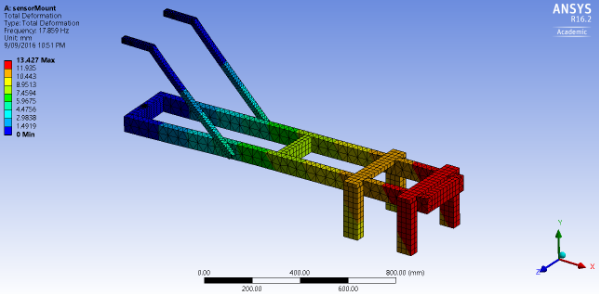
\includegraphics[width=0.8\textwidth]{4-DetailedDesign/VibeAnal.PNG}
\centering
\caption{Sensor mount frame design vibrational analysis} \figlabel{Finalframeansys}
\end{figure} 

The addition of the metal detector to the frame resulted in fundamental frequencies of 13.647, 14.573 and 31.913 Hz with a maximum deflection of 9.9417 mm. The addition of the weight of the metal detector acts to dampen the fundamental frequency as expected. This same damping can be seen from the theoretical results for the cantilever beam with the added end weight.

Variations in sensor arrangements that could be installed would result in different fundamental frequencies due to the changing damping effects. This can be accounted for by increasing of decreasing the length of the frame to change the fundamental frequency to one that is desired. The frame design can be tuned to a specific fundamental frequency through the alteration of its design and end weight.   

\subsection{Manufacturing}
The processes required in the construction the sensor mount consisted of wood work and metal work. Wooden dowels were used to join the sections together near the metal detector as no metallic objects were allowed near it. Supports for the metal detector were made out of four nylon rods that connect to horizontal wooden supports. Two acrylic boards were made to encase the metal detector to act as both a safety protector and a mounting device for the nylon rods. As the sensor was a loaned piece of equipment, no modifications or damages were allowed  resulting in the need for the acrylic case. The requirement for variation in the height of the sensor was satisfied by the use of the nylon rods, the length and subsequently the height of the sensor off the ground could be altered by varying the length of the rods and supports. Another benefit to using the nylon rods is that in the case that the quad bike were to hit something, the metal detector would not break, instead the nylon rods would shear resulting in no damage to the sensor.
\Figref{ManufactoredFrame} shows the completed manufactured frame with the sensors attached. 
\begin{figure}[ht]
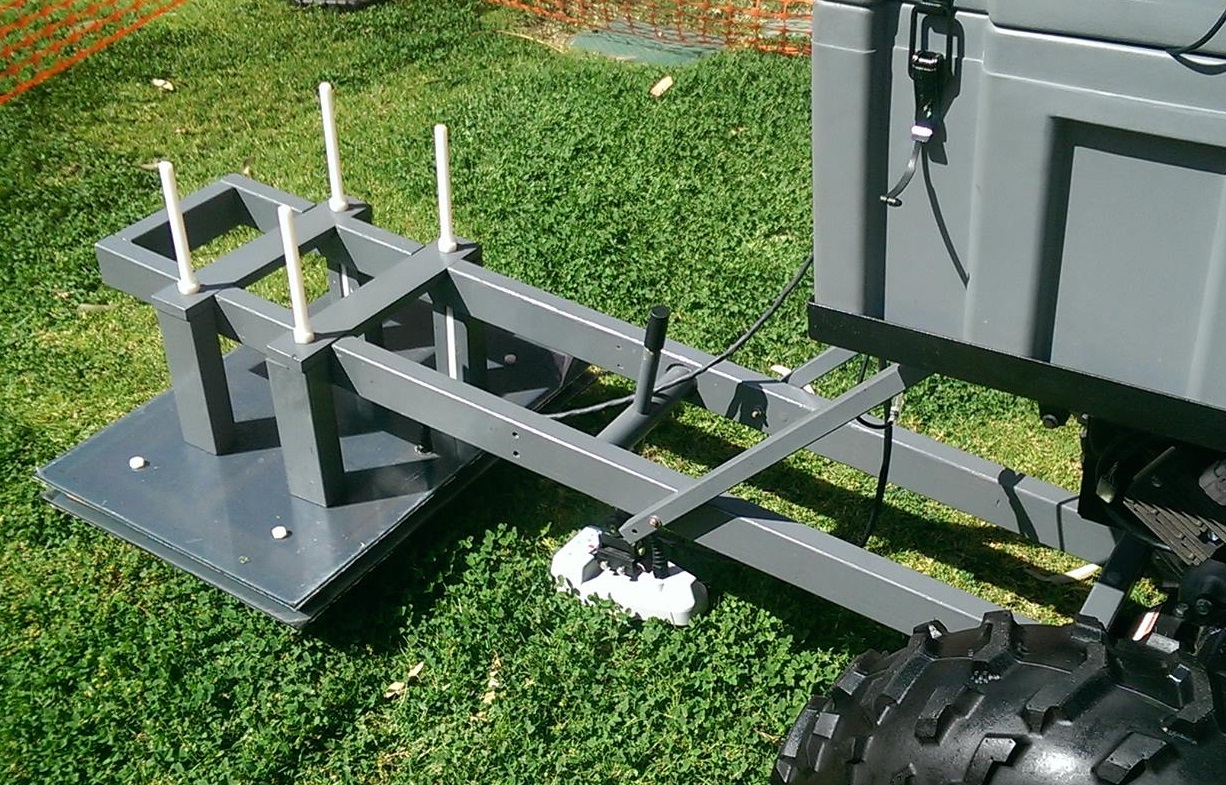
\includegraphics[width=0.8\textwidth]{4-DetailedDesign/QuadBikeFinalFrame.jpg}
\centering
\caption{Manufactured and mounted frame with sensors attached} \figlabel{ManufactoredFrame}
\end{figure}

The installation of the GPR had to fulfil the requirements outlined for the correct operation of the sensor. The main requirement being the operating distance off the ground. A telescoping mounting arm was utilised whereby any changes in the slope of the terrain would allow for the GPR head to maintain within contact with the ground satisfying the sensors operating requirement. This was attached in line with the central metal detector panel through the use of a PVC pipe to reduce misalignment that would be present during turns. With the pipe being fixed to the frame using silicon glue, the flexibility of the join would ensure that the GPR would not get damaged if it were to hit a object, as the join would flex and bend instead of the load being felt by the sensor.  
  
\subsubsection{Quad bike Vibration testing}
Accelerometers were used to measure the amount of vibration present on the quad bike and the sensor frame during operation. Measurements from inside the storage compartment and the end of the frame were taken through a variation of throttle positions. \Figref{Vibrationtest} shows the vibrational frequencies experienced by the frame due to the quad bike vibrations. It can be seen that there is a peak in vibrational frequency at roughly 15 Hz which corresponds to the calculated fundamental frequency for the frame. Figure XX shows the vibrational frequency for the quad bike that excites the frame. Due to the accelerometer    

\begin{figure}[ht]
\centerline{
\begin{tabular}{cc}
\subfloat[Power spectrum of accelerometer data on idling quad bike]{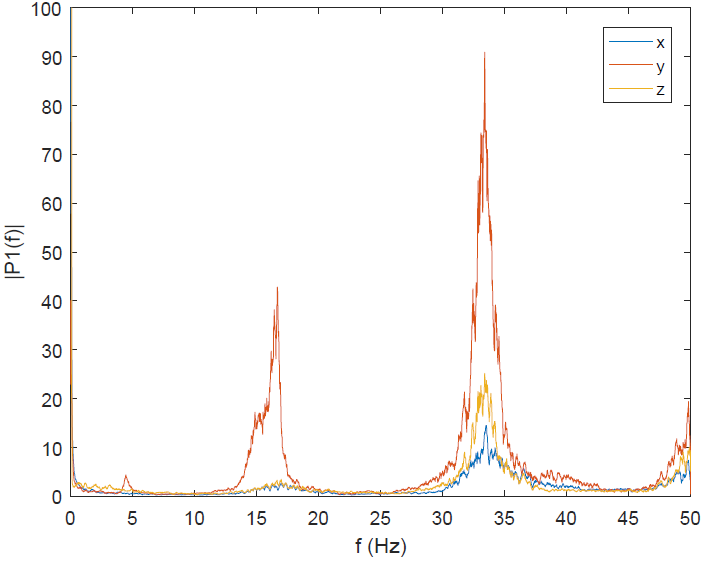
\includegraphics[height=0.4\textwidth]{4-DetailedDesign/quadIdle}} 
   & \subfloat[Power spectrum of accelerometer data on throttling quad bike]{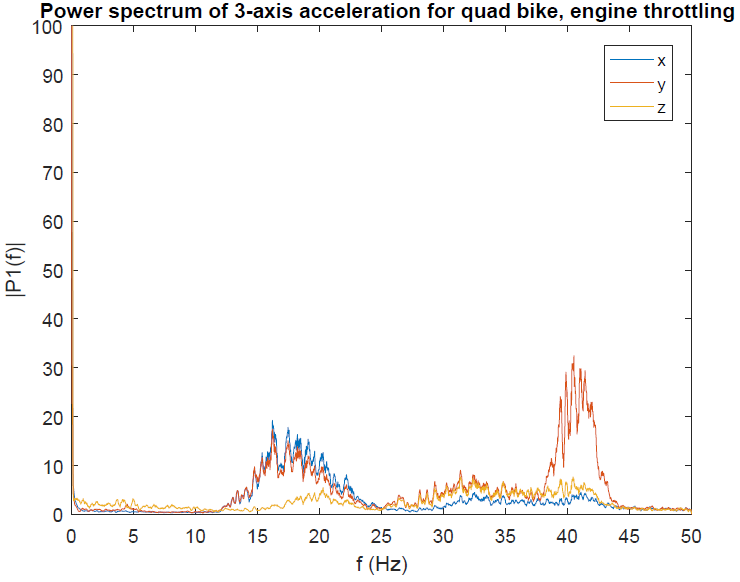
\includegraphics[height=0.4\textwidth]{4-DetailedDesign/quadThrottle}}\\
\subfloat[Power spectrum of accelerometer data on sensor mount for idling quad bike]{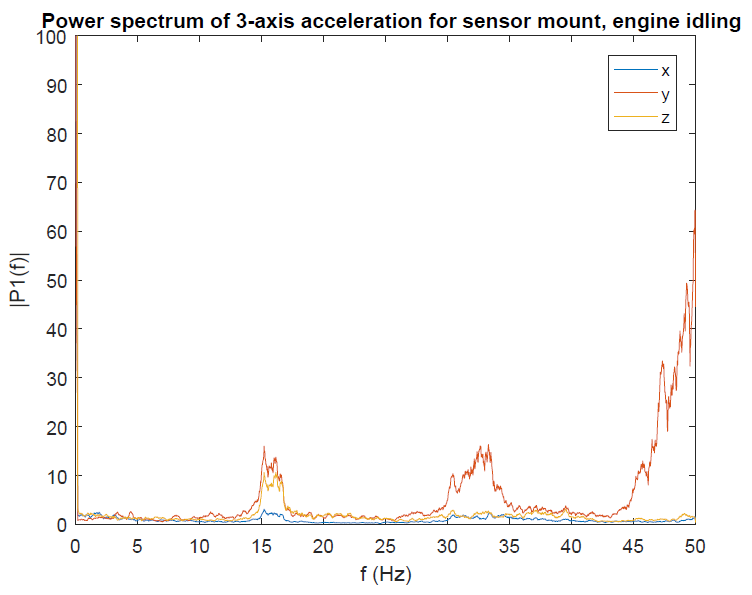
\includegraphics[height=0.4\textwidth]{4-DetailedDesign/mountIdle}}
   & \subfloat[Power spectrum of accelerometer data on sensor mount for throttling quad bike]{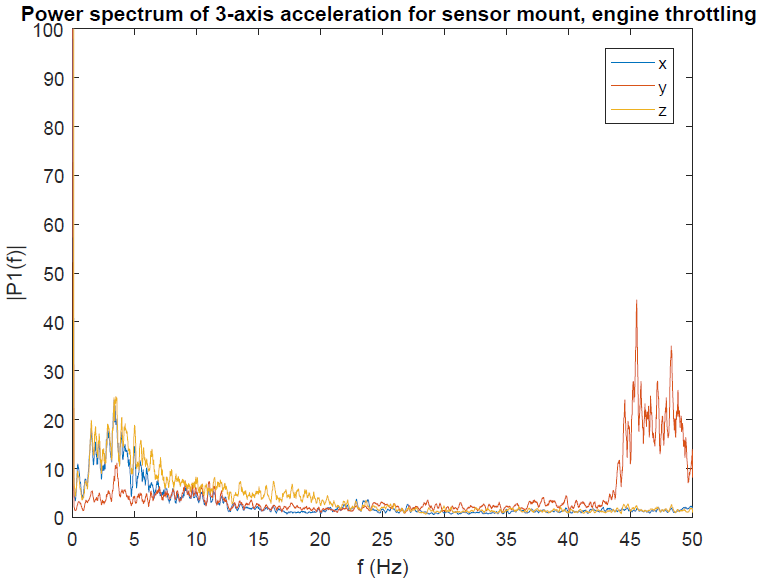
\includegraphics[height=0.4\textwidth]{4-DetailedDesign/mountThrottle}}
\end{tabular}}
\caption{Sensor mount Vibrational testing x is forwards, y is transverse and z is horizontal vibration direction. All directions are relative to rear wheel steering}
\figlabel{Vibrationtest}
\end{figure}

The vibrational tests from inside the quad bike storage tray resulted in the data as seen in Figure XXX. Due to the accelerometer used only having a sampling rate of 100 Hz, the highest frequency that was able to be resolved was up to was 50 Hz. This results in no peaks for the quad bike vibrations as the fundamental vibrational mode was greater than 50 Hz. This leads to the conclusion that the operation of the quad bike would not result in the fundamental mode of the sensor frame being excited. The mode would only be excited for a brief moment during start up and shut down procedures of the engine as the vibrations passed through the harmonic range of the frame.

\section{Electronics}
The electronics hardware to be used for the project will fit in the categories as described in the Conceptual Design. The custom electronics work pre-existing on the quad bike supplied by the DSTG meets the requirements for the COTS bespoke electronics, providing digital interfaces to the actuators and sensors attached to the platform. The need for replacement or improvement of any of these electronics will be determined after testing has been completed on the supplied vehicle and their performance has been evaluated.

As the electronics system does not have particularly strict requirements for part selection, and due to the COTS equipment being mostly interchangeable with little effect on appropriateness for the project, the electronics hardware has been chosen on a basis of what is most readily available to the project and most familiar to the project members. This choice reduces time spent in the design stage and allows for a rapid development process to commence as early as possible.

The central processing hardware will be provided by a Windows based desktop computer supplied by the University of Adelaide. A Windows device has been chosen to be able to make use of the provided drivers for the GPR system which are only compatible with 32-bit Windows machines. The selected device has WiFi communications capabilities and dedicated serial communications ports, allowing easy communications to a microcontroller device providing low level I/O.

The microcontroller selected is an Arduino Mega 2560 board, chosen for its cost, availability and fast development time. This board has considerable I/O capabilities that exceed the requirements for the project, but allow for future expansion of sensors and ensures that I/O limitations will not be a concern. The microcontroller will be connected to the desktop computer via the serial port as mentioned above.

\section{Software}
\textcolor{red}{Intro for this section}
\seclabel{detailedSoftware}

\subsection{Software architecture}
\seclabel{detailedSoftwareArchitecture}
Due to the experimental nature of much of this project, and with the short timeframe available, it was anticipated that moving goalposts would have a significant impact on the development of this project. As project complexities could not be fully understood in the design stage, an Agile software development strategy was adopted. Under this routine, strict determinations of the software design were not detailed at the outset of development. The agile practice involves delivering incremental improvements to a working software and constantly assessing progress to identify software features that do not perform as anticipated or are more difficult than planned to implement. The agile strategy welcomes changing software requirements even late in development to accommodate the outcomes of these evaluations.
As such, the software design prior to the development phase included only the outline description of a completed system, with software subsystems partially detailed. Full detail of these subsystems or additional systems would be determined during the development phase after assessment of progress and performance. This initial outline is shown below in \textcolor{red}{figure XXX}.

\textcolor{red}{XXxXX figure XXXxXXxX}

To allow for the most rapid development, the primary focus for the initial portion of the development phase was to complete the Central object and the Window and Data Logging objects. These were chosen due to the anticipated low complexity for these systems, and the dependency other systems would have regarding these systems. The full Software Requirements Specification, and Software Design Document – which were completed as part of the iterative agile development process and reflect the design changes made during development – are presented in \textcolor{red}{Appendix XXX}.


\subsection{Virtual platform}
\seclabel{detailedVP}
The virtual platform was designed to test software implementations for communications, automation, and navigation software. As shown in \Figref{virtualPlatformPic}, the virtual platform displays a graphical representation of the quad bike as it traverses a given path, graphs showing the actuator states of the wheel encoder, steering, gear, and throttle subsystems, ground penetrating radar output, and the metal detector output.
\begin{figure}[ht]
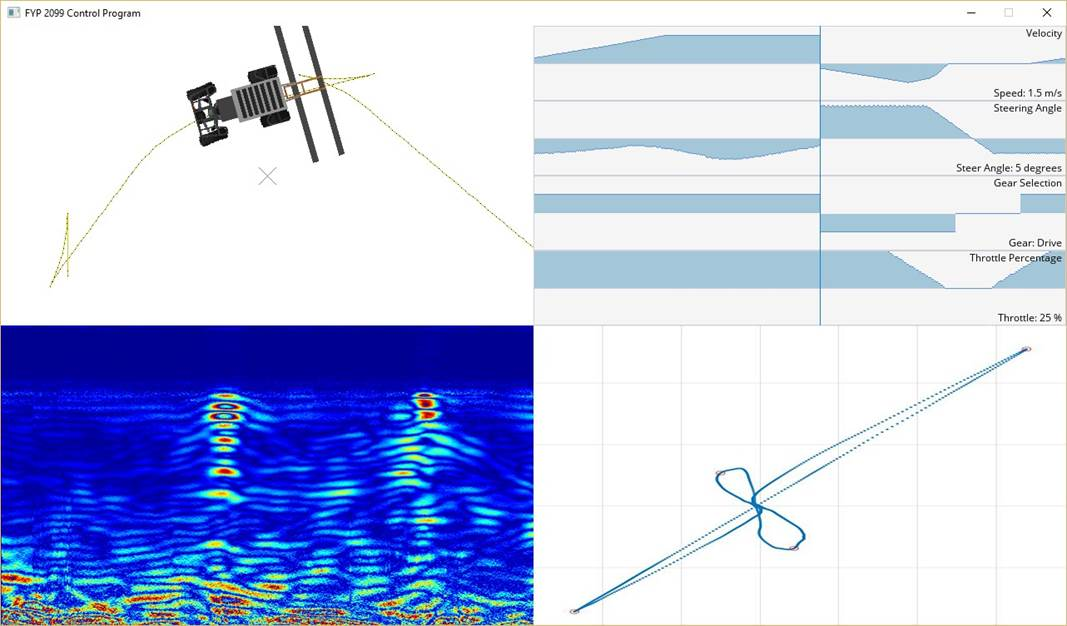
\includegraphics[width=\textwidth]{4-DetailedDesign/virtualPlatform.jpg}
\centering
\caption[Virtual platform display window]{Virtual platform: graphical representation (top left), actuator states (top right), GPR output (bottom left), MD output (bottom right)} \figlabel{virtualPlatformPic}
\end{figure}
The user also has the option to display, on the graphical representation, the positional sensor data as seen in \Figref{virtualPlatformDataPic}. Note that the IMU heading is in the incorrect direction as the initialised heading is unknown.
\begin{figure}[ht]
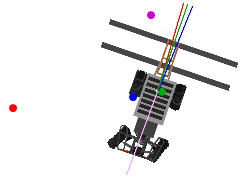
\includegraphics[]{4-DetailedDesign/dataVisibleVirtualPlatform.PNG}
\centering
\caption[Virtual platform graphical representation]{Virtual platform graphical representation showing sensor data, GPS (blue), kinematic equations (red), Kalman Filtered (green), and IMU (pink). Purple is the goal waypoint.} \figlabel{virtualPlatformDataPic}
\end{figure}
The virtual platform is initialised as soon as any waypoints are sent which can be navigated. It takes user waypoints which are passed to the virtual platform, are subdivided and sent to the automation code to begin navigation.

\subsection{Tablet application}
\seclabel{detailedTabletApp}
The tablet application was designed to meet to project goal of allowing easy usage of the entire mine detection system by an unskilled operator. To this end, the design of the UI is focussed towards providing the most user friendly interface possible, in preference to displaying the most informative data. The expectation is that an unskilled operator is unlikely to be able to form meaningful conclusions from an output displaying the unprocessed data, and as a result this information has been omitted from the design of the operator’s device. 

Key components of the UI are the map display, and the controls pane. The map display is the primary method of displaying information about the system to the operator, and as a result is permanently shown in a prominent location. The emergency stop button is the only other UI item which is permanently available, which for safety reasons is always prominently displayed and readily accessible. The controls pane is split into three windows, which each correspond to a common control theme – manual controls, automation and navigation controls, and communications controls. These distinctions were made as it allows for the control buttons to be larger and more informative, and readily distinguishes clusters of controls which serve similar functions. 

The map display shows the current locations of all of the paths and zones defined on the tablet, as well as an indicator showing the current geographical location of the remote device. Under autonomous conditions, the map display will show a trail indicating the path which has been covered by the platform during the scan. Upon detection of an object, this will be displayed on the map showing location, and confidence of the detected object being a mine. Above a certain confidence threshold, the remote platform will halt, and the operator will be prompted.

The communications tab provides all of the required interfaces to establish, maintain and assert communications with the remote platform. This will be the primary view displayed to the operator, as it must be completed before control of the platform can be achieved. Under normal operations, once connected it will not be necessary for an operator to return to the communications tab.

The automation and navigation tab provides all of the controls for defining routes and zones on the tablet device, including synchronising these paths with the remote platform. The controls for initiating and pausing autonomous motion, as well as determining the current state of the autonomous systems, are displayed here.

The manual control tab provides a joystick with which an operator can control the remote platform without needing to define a path. It is anticipated that this will primarily be used for positioning the remote platform prior to commencing a scan, such as driving the platform off a trailer, or navigating a complex terrain. This tab also displays information about the current speed and heading of the remote platform. 



\subsection{Communications}
\seclabel{detailedComms}
Communications between all aspects of the system will be controlled by a system of packets. Each packet has a custom structure created specifically for this project, and is consistent irrespective of communications protocol used. The use of this system means that packets created on the operator’s device can be transmitted to the Arduino via the PC and be interpreted correctly, without needing intermediate processing. The structure of each packet is as follows:
\begin{itemize}
\item Packet ID: A single byte identifying the purpose of this packet.
\item Length: A single byte indicating the length (in bytes) of this transmission
\item Data: A stream of bytes (in multiples of 4) corresponding to an array of IEEE 754 format floating point numbers
\end{itemize}
Using this system a technical limit of up to 63 floats can be transmitted in a single packet. The vast majority of packets will have either zero associated data or only a single data point, and in practical application it is unlikely that this amount of data will be required in a single transmission. The full detail of packet structure is provided in Appendix XXX. 



\end{document}